\documentclass[10pt]{beamer}

\usepackage[french]{babel}
\usepackage[utf8]{inputenc}
\usepackage{sansmathfonts} % Set sans-serif font (with small caps option and math option)
\usepackage{slantsc}% access different-shaped small-caps fonts
\usepackage[french, showdow]{datetime2}% permet d'avoir la commande \Today qui affiche la date du jour

% \usepackage[colorlinks = true,
%             linkcolor = blue,
%             urlcolor  = blue,
%             citecolor = blue,
%             anchorcolor = blue]{hyperref}
            
% Packages pour les maths
\usepackage{amsthm}
\usepackage{amsmath}
\usepackage{amssymb}
\usepackage{mathrsfs}
\usepackage{mathabx}


\usepackage{tikz}
\usetikzlibrary{patterns}
\usetikzlibrary{shapes.geometric, arrows.meta}
\usetikzlibrary{positioning,calc}

% Rappel
\newtheoremstyle{dotlessRappel}{}{}{}{}{\color{black}\bfseries}{}{ }{}
\theoremstyle{dotlessRappel}
\newtheorem*{rappel}{Rappel}


% Proposition
\newtheoremstyle{dotlessProp}{}{}{}{}{\color{black}\bfseries}{}{ }{}
\theoremstyle{dotlessProp}
\newtheorem*{proposition}{Proposition}

% Remarque
\newtheoremstyle{dotlessRemq}%    <name>
{\topsep}%   <space above>
{\topsep}%   <space below>
{\itshape}%  <body font>
{}%          <indent amount>
{\bfseries}% <Theorem head font>
{}%          <punctuation after theorem head>
{ }%{\newline}%  <space after theorem head> (default .5em)
{}%          <Theorem head spec>
\theoremstyle{dotlessRemq}
\newtheorem*{remq}{Remarque}

% Theorème
\newtheoremstyle{dotlessThm}{}{}{}{}{\color{teal}\bfseries}{}{ }{}
\theoremstyle{dotlessThm}
\newtheorem*{thm}{Théorème}

% Example
\newtheoremstyle{dotlessEx}{}{}{}{}{\color{vert}\bfseries}{}{ }{}
\theoremstyle{dotlessEx}
\newtheorem*{ex}{Exemple}
\newtheorem*{exs}{Exemples}

% Definition
\newtheoremstyle{dotlessDef}{}{}{}{}{\color{lipstick}\bfseries}{}{ }{}
\theoremstyle{dotlessDef}
\newtheorem*{mydefinition}{Définition}

\usetheme[progressbar=frametitle]{metropolis}
\usecolortheme{disco}
\setbeamertemplate{frame footer}{\insertshorttitle~-~\insertshortauthor}

\usepackage{appendixnumberbeamer}
\usepackage{booktabs}
\usepackage[scale=2]{ccicons}

\usepackage{xspace}

\title{Bases de données NoSQL}
% \subtitle{Introduction au NoSQL}
\date{\Today}
\author{Alanna \textsc{Devlin Génin}}
\institute{IUT Rives de Seine - BUT Science des Données - Parcours VCOD}
\titlegraphic{\hfill
\includegraphics[height=1.5cm]{img/db-transfer.png}}
% 
\includegraphics[height=1cm]{img/logos/logo-iut.jpg}

% \makeatletter
% \tikzset{
%     database/.style={
%         path picture={
%             \draw (0, 1.5*\database@segmentheight) circle [x radius=\database@radius,y radius=\database@aspectratio*\database@radius];
%             \draw (-\database@radius, 0.5*\database@segmentheight) arc [start angle=180,end angle=360,x radius=\database@radius, y radius=\database@aspectratio*\database@radius];
%             \draw (-\database@radius,-0.5*\database@segmentheight) arc [start angle=180,end angle=360,x radius=\database@radius, y radius=\database@aspectratio*\database@radius];
%             \draw (-\database@radius,1.5*\database@segmentheight) -- ++(0,-3*\database@segmentheight) arc [start angle=180,end angle=360,x radius=\database@radius, y radius=\database@aspectratio*\database@radius] -- ++(0,3*\database@segmentheight);
%         },
%         minimum width=2*\database@radius + \pgflinewidth,
%         minimum height=3*\database@segmentheight + 2*\database@aspectratio*\database@radius + \pgflinewidth,
%     },
%     database segment height/.store in=\database@segmentheight,
%     database radius/.store in=\database@radius,
%     database aspect ratio/.store in=\database@aspectratio,
%     database segment height=0.1cm,
%     database radius=0.25cm,
%     database aspect ratio=0.35,
% }
% \makeatother

% Draw a database
\makeatletter
\tikzset{
    database top segment style/.style={draw},
    database middle segment style/.style={draw},
    database bottom segment style/.style={draw},
    database/.style={
        path picture={
            \path [database bottom segment style]
                (-\db@r,-0.5*\db@sh) 
                -- ++(0,-1*\db@sh) 
                arc [start angle=180, end angle=360,
                    x radius=\db@r, y radius=\db@ar*\db@r]
                -- ++(0,1*\db@sh)
                arc [start angle=360, end angle=180,
                    x radius=\db@r, y radius=\db@ar*\db@r];
            \path [database middle segment style]
                (-\db@r,0.5*\db@sh) 
                -- ++(0,-1*\db@sh) 
                arc [start angle=180, end angle=360,
                    x radius=\db@r, y radius=\db@ar*\db@r]
                -- ++(0,1*\db@sh)
                arc [start angle=360, end angle=180,
                    x radius=\db@r, y radius=\db@ar*\db@r];
            \path [database top segment style]
                (-\db@r,1.5*\db@sh) 
                -- ++(0,-1*\db@sh) 
                arc [start angle=180, end angle=360,
                    x radius=\db@r, y radius=\db@ar*\db@r]
                -- ++(0,1*\db@sh)
                arc [start angle=360, end angle=180,
                    x radius=\db@r, y radius=\db@ar*\db@r];
            \path [database top segment style]
                (0, 1.5*\db@sh) circle [x radius=\db@r, y radius=\db@ar*\db@r];
        },
        minimum width=2*\db@r + \pgflinewidth,
        minimum height=3*\db@sh + 2*\db@ar*\db@r + \pgflinewidth,
    },
    database segment height/.store in=\db@sh,
    database radius/.store in=\db@r,
    database aspect ratio/.store in=\db@ar,
    database segment height=0.1cm,
    database radius=0.25cm,
    database aspect ratio=0.35,
    database top segment/.style={
        database top segment style/.append style={#1}},
    database middle segment/.style={
        database middle segment style/.append style={#1}},
    database bottom segment/.style={
        database bottom segment style/.append style={#1}}
}
\makeatother

% Draw a single disk database
\makeatletter
\tikzset{
    disk segment style/.style={draw},
    disk/.style={
        path picture={
            \path [disk segment style]
                (-\db@r,1.5*\db@sh) 
                -- ++(0,-1*\db@sh) 
                arc [start angle=180, end angle=360,
                    x radius=\db@r, y radius=\db@ar*\db@r]
                -- ++(0,1*\db@sh)
                arc [start angle=360, end angle=180,
                    x radius=\db@r, y radius=\db@ar*\db@r];
            \path [disk segment style]
                (0, 1.5*\db@sh) circle [x radius=\db@r, y radius=\db@ar*\db@r];
        },
        minimum width=2*\db@r + \pgflinewidth,
        minimum height=3*\db@sh + 2*\db@ar*\db@r + \pgflinewidth,
    },
    disk segment height/.store in=\db@sh,
    disk radius/.store in=\db@r,
    disk aspect ratio/.store in=\db@ar,
    disk segment height=0.1cm,
    disk radius=0.25cm,
    disk aspect ratio=0.35,
    disk segment/.style={
        disk segment style/.append style={#1}}
}
\makeatother


% Define a reusable node for a stack of files
\newcommand{\filestack}{
    \begin{tikzpicture}
        \def\corner{0.15in}
        \def\cornerradius{0.02in}
        \def\lwidth{0.02in}
        \def\h{1.1in}
        \def\w{0.85in}
        \def\nline{10}
        \def\iconmargin{0.1in}
        \def\topmargin{0.3in}
        \foreach[count=\i] \filename in {Shard 5, Shard 4, Shard 3, Shard 2, Shard 1}
        {
        \coordinate (nw) at ($(-0.05in*\i,-0.15in*\i)$);
        \coordinate (ne0) at ($(nw) + (\w, 0)$);
        \coordinate (ne1) at ($(ne0) - (\corner, 0)$);
        \coordinate (ne2) at ($(ne0) - (0, \corner)$);
        \coordinate (se) at ($(ne0) + (0, -\h)$); 
        \filldraw [-, line width = \lwidth, fill=white] (nw) -- (ne1) -- (ne2)
            [rounded corners=\cornerradius]--(se) -- (nw|-se) -- cycle;
        \draw [-, line width = \lwidth] (ne1) [rounded corners=\cornerradius]-- (ne1|-ne2) -- (ne2);
        \node [anchor=north west] at (nw) {\scriptsize \tt \filename};
        \foreach \k in {1,...,\nline}
        {
            \draw [-, line width = \lwidth, line cap=round] 
            ($(nw|-se) + (\iconmargin,\iconmargin) + (0,{(\k-1)/(\nline-1)*(\h - \iconmargin - \topmargin)})$)
                -- ++ ($(\w,0) - 2*(\iconmargin,0)$);
        }
        }
    \end{tikzpicture}
}

% ------------------------------------------------------

\begin{document}

% \maketitle
\begin{frame}
   \tikz [remember picture,overlay]
    \node at
        ([yshift=0.6cm,xshift=3.9cm]current page.south) 
        %or: (current page.center)
        {
\includegraphics[height=1cm]{img/logos/logo-iut.jpg}};
   \titlepage
\end{frame}

% \begin{frame}{Programme}

\begin{itemize}
    \item Introduction au NoSQL
    \item Caractéristiques principales des bases de données NoSQL
    \item Typologie NoSQL
    \item Avantages et inconvénients
    \item Cas d'usages
\end{itemize}

\end{frame}


\begin{frame}{Planning}
    
    7 séances de 3 heures\\

    \begin{itemize}
        \item Séance 1 : CM (lundi 9 septembre)
        \item Séance 2 : TP (jeudi 12 septembre)
        \item Séance 3 : TP (vendredi 13 septembre)
        \item Séance 4 : TP (mardi 24 septembre)
        \item Séance 5 : TP (vendredi 27 septembre)
        \item Séance 6 : TP (vendredi 11 octobre)
        \item Séance 7 : TP (vendredi 8 novembre)

    \end{itemize}
\end{frame}

\begin{frame}{Evaluation}
    
QCM avec une ou deux questions ouvertes (30 minutes)

Rendu de TP

\end{frame}



% \begin{frame}{Mon parcours académique}

    \begin{tikzpicture}
        \begin{scope}
            \clip (0,0)  circle (2cm) ;
            \node[anchor=center] (me) {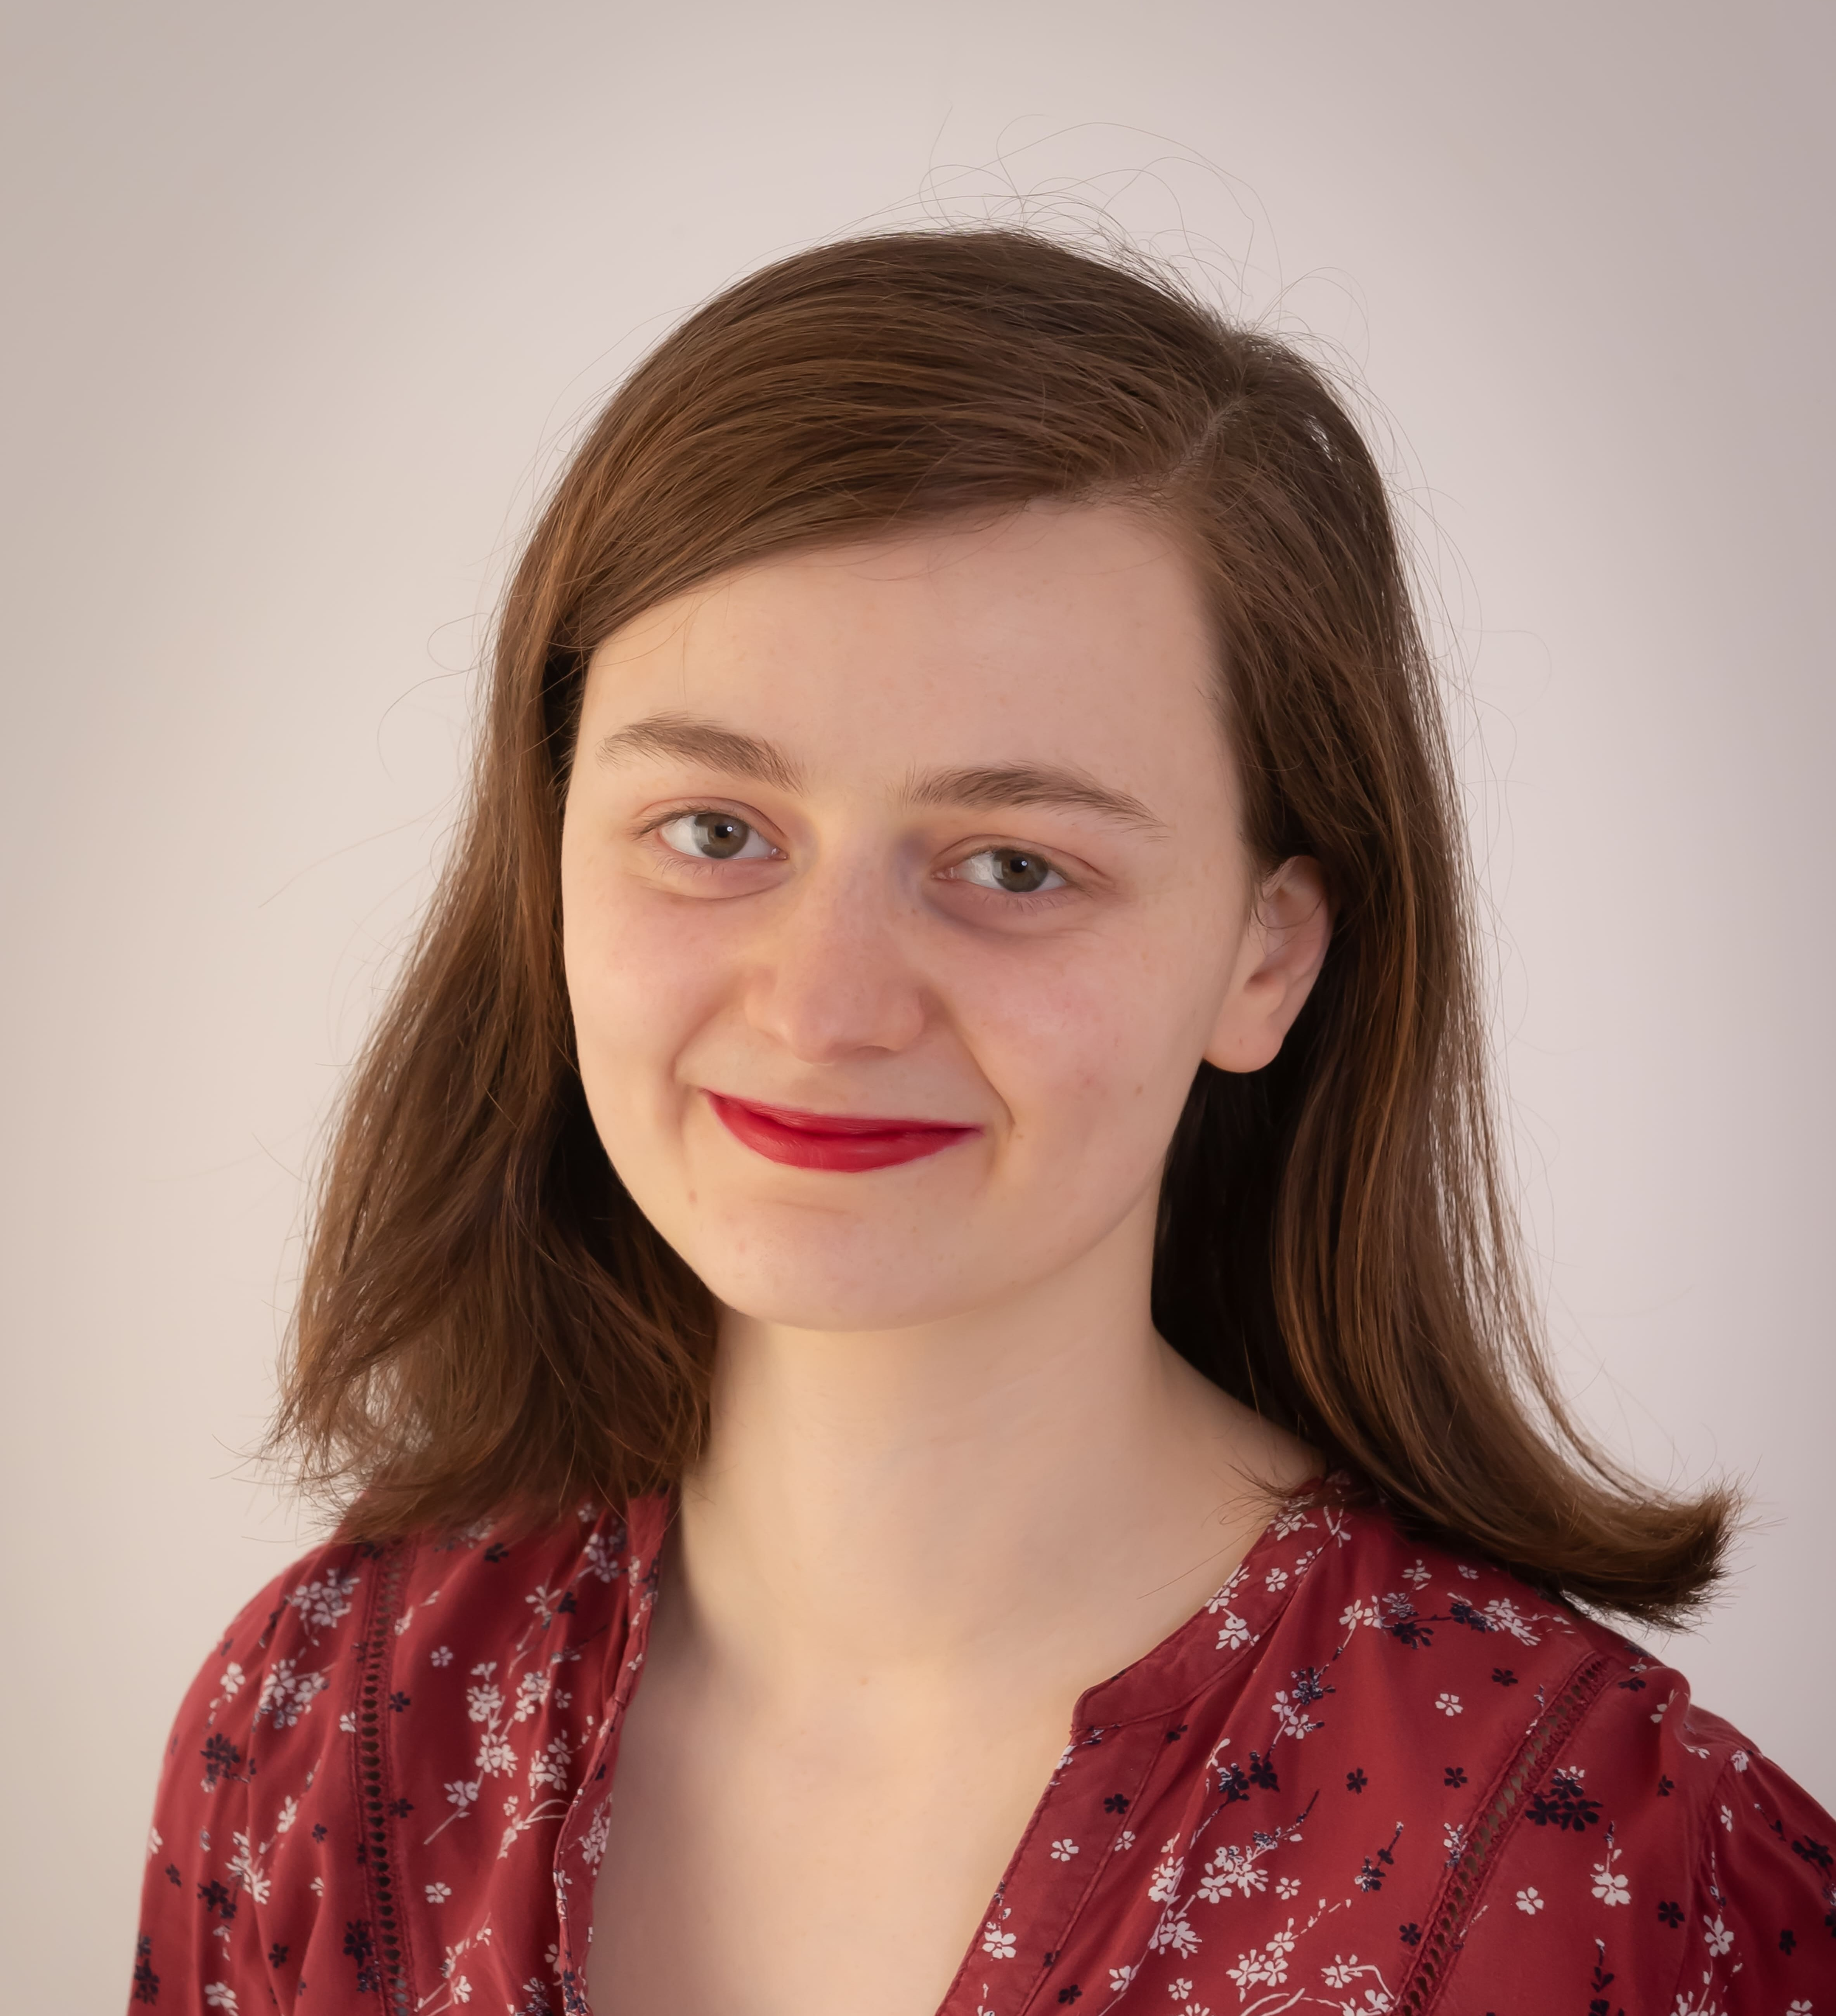
\includegraphics[width=4cm]{img/alanna.jpg}} ; 
        \end{scope}    
        
        % Position stid in the top-left corner of me
        \node[xshift=5.5cm,yshift=3.5cm,anchor=south east] at (me.south east) (stid) {
\includegraphics[width=4cm]{img/logos/logo-stid.jpg}};
        \node[anchor=south,yshift=-0.2cm] at (stid.south) (stidtexte) {DUT STID en formation initiale};
        \node[anchor=south,yshift=-0.4cm] at (stidtexte.south) (stage) {Stage RShiny au Cnam};
        
        % Position ensai below stid
        \node[anchor=south,yshift=-3.5cm] at (stid.south) (ensai) {
\includegraphics[width=4cm]{img/logos/logo-ensai.png}};
        \node[anchor=south,yshift=-0.2cm] at (ensai.south) (ensaitexte) {École ingénieur ENSAI};
        \node[anchor=south,yshift=-0.4cm] at (ensaitexte.south) {Filière Data Science et Data Engineering};
        
    \end{tikzpicture}
\end{frame}

\begin{frame}{Mon parcours professionnel}
    
    \begin{tikzpicture}
        \begin{scope}
            \clip (0,0)  circle (2cm) ;
            \node[anchor=center] (me) {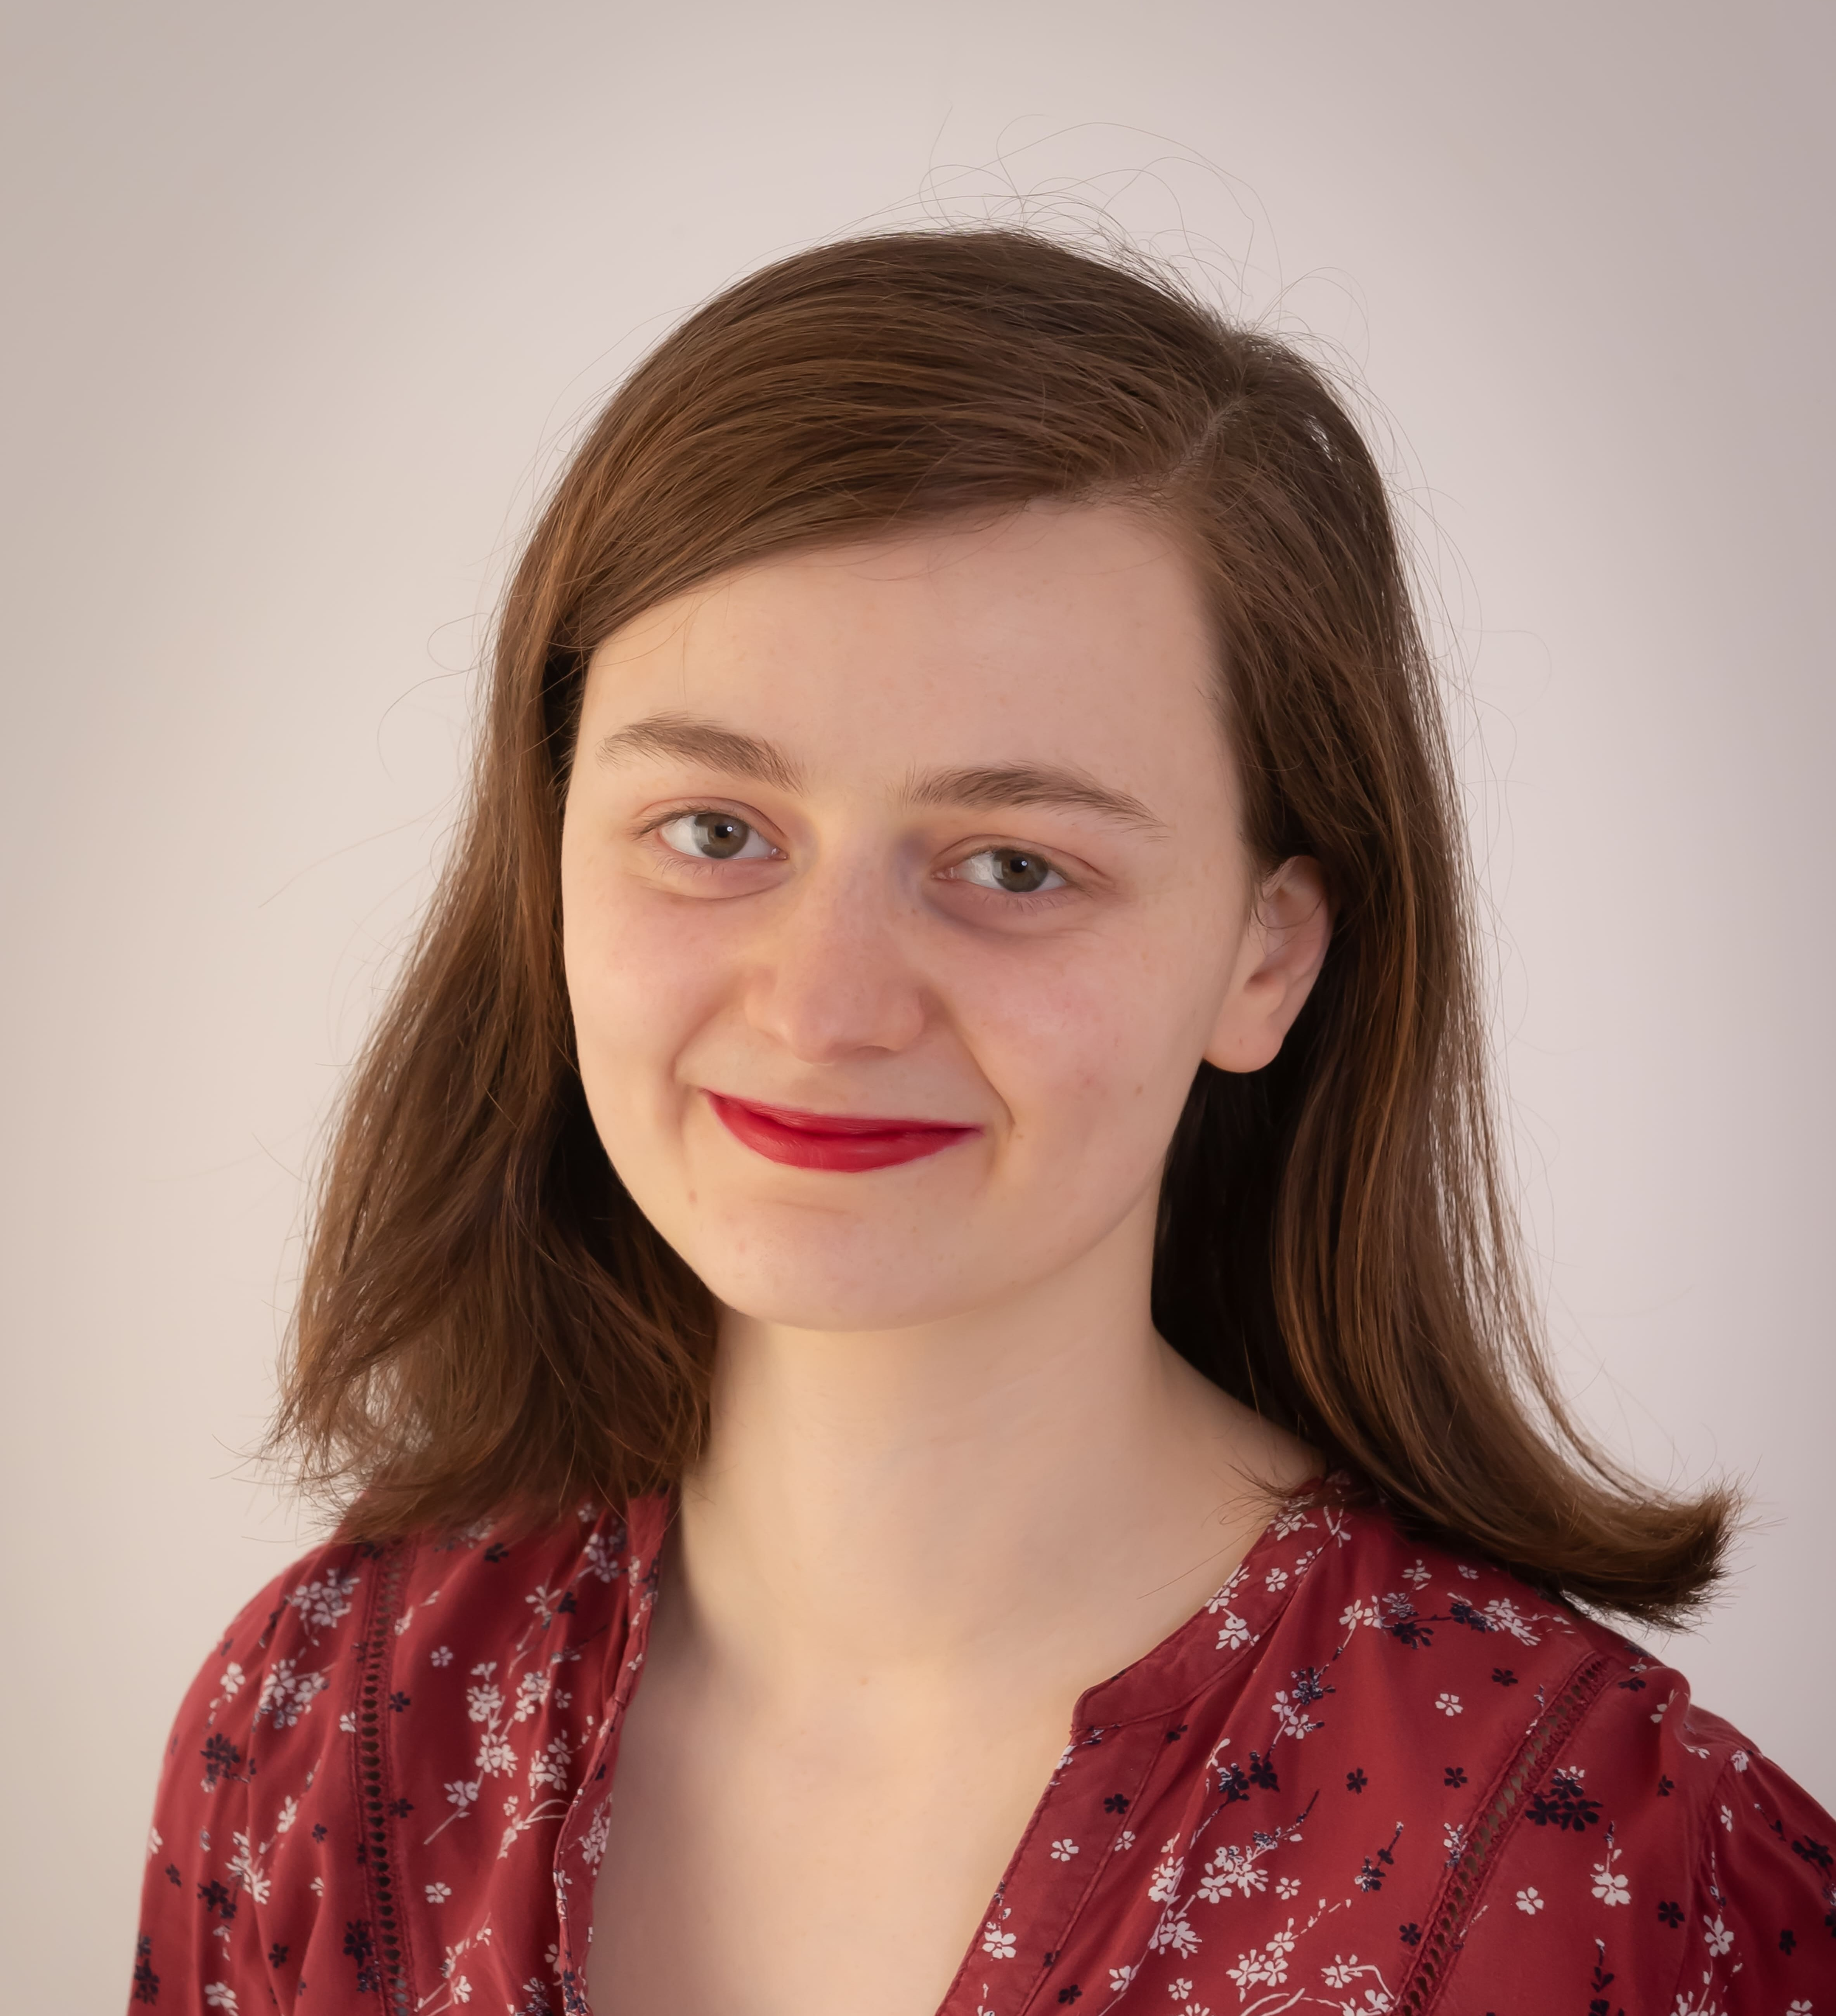
\includegraphics[width=4cm]{img/alanna.jpg}} ; 
        \end{scope}    
        
        % LBC
        \node[xshift=3.5cm] at (me.east) (lbc) {
\includegraphics[width=5cm]{img/logos/logo-littlebigcode.png}};
        \node[anchor=south,yshift=-0.5cm] at (lbc.south) (stage) {Stage fin d'études};
        \node[anchor=south,yshift=-0.4cm] at (stage.south) (poste) {Data Engineer depuis 1 an et demi};

    \end{tikzpicture}


\end{frame}


\begin{frame}{Contact}

Si vous avez des questions n'hésitez pas à me contacter :

\href{mailto:alannadevlingenin@gmail.com}{alannadevlingenin@gmail.com}

\end{frame}


% \begin{frame}{Sommaire}
%   \setbeamertemplate{section in toc}[sections numbered]
%   \tableofcontents%[hideallsubsections]
% \end{frame}

% \section{Historique}

\begin{frame}{Historique}

    \begin{itemize}
        \item 2009 : Eric Evans, Johan Oskarsson et Dwight Merriman organisent un événement à San Francisco
        \item 2011 : Johan Oskarsson crée le terme NoSQL
        \item 2012 : Johan Oskarsson organise la première conférence NoSQL à San Francisco
        \item 2013 : Johan Oskarsson organise la première conférence NoSQL en Europe
    \end{itemize}

\end{frame}


% \section{Introduction au NoSQL}

\begin{frame}{Pourquoi NoSQL ?}

    \begin{itemize}
        \item Besoin de stocker et de traiter des données massives
        \item Besoin de scalabilité
        \item Besoin de haute disponibilité
        \item Besoin de réplication
        \item Besoin de partitionnement
        \item Besoin d'indexation
        \item Besoin de transactions
    \end{itemize}

\end{frame}

\begin{frame}{Mais que signifie NoSQL ?}

    NoSQL signifie Not Only SQL ou No SQL.

\end{frame}

\begin{frame}{Définition}

    Johan Oskarsson définit NoSQL comme un terme générique pour désigner les bases de données qui ne sont pas des bases de données relationnelles.

\end{frame}


\begin{frame}{NewSQL}

    NewSQL est un terme générique pour désigner les bases de données qui sont des bases de données relationnelles mais qui sont conçues pour être distribuées.

    Examples : Google Spanner, CockroachDB, NuoDB, VoltDB, MemSQL, Clustrix, etc.
\end{frame}

\begin{frame}[standout]
    
Time for Kahoot!

\end{frame}
\section{Concepts fondamentaux}

% \begin{frame}{Caractéristiques principales du NoSQL}

%     \begin{itemize}
%         \item Schéma flexible
%         \item Scalabilité
%         \item Haute disponibilité
%         \item Réplication
%         \item Partitionnement
%         \item Indexation
%         \item Transactions
%     \end{itemize}
% \end{frame}

% \begin{frame}{Schéma flexible}

%     \begin{itemize}
%         \item Schéma fixe : SQL
%         \item Schéma flexible : NoSQL
%     \end{itemize}

% \end{frame}

% \begin{frame}{Scalabilité}

%     Scalabilité horizontale : Ajout de machines pour augmenter la capacité de stockage et de traitement

%     Scalabilité verticale : Ajout de ressources (CPU, RAM, Disque) sur une machine existante

% \end{frame}

% \begin{frame}{Haute disponibilité}

%     Garantir un service disponible en tout temps

%     \begin{itemize}
%         \item Réplication
%         \item Partitionnement
%         \item Tolérance aux pannes
%     \end{itemize}

% \end{frame}

% \begin{frame}{Réplication}

%     \begin{itemize}
%         \item Réplication synchrone
%         \item Réplication asynchrone
%         \item Réplication multi-maître
%     \end{itemize}

% \end{frame}

% \begin{frame}{Partitionnement}

%     Partitionnement ou sharding : séparer les données en plusieurs chunks

%     Faire diagramme avec les différentes stratégies de partitionnement

%     \begin{itemize}
%         \item Partitionnement par clé
%         \item Partitionnement par plage
%         \item Partitionnement par hachage
%     \end{itemize}

% \end{frame}

\begin{frame}{Sharding (partitionnement horizontal)}

    % \begin{tikzpicture}[line width=1pt]
    %     \node[database,label=below:DB,database radius=1cm,database segment height=0.5cm] at (3,0) {};
    % \end{tikzpicture}

    \begin{tikzpicture}[line width=1pt]
        \node[database,ultra thick,database radius=1cm,database segment height=0.5cm, database top segment={draw=black,fill=customgreen}, database middle segment={draw=black,fill=customgreen}, database bottom segment={draw=black,fill=customgreen}] at (0,0) {};
        \node[database,ultra thick,database radius=1cm,database segment height=0.5cm, database top segment={draw=black,fill=customblue}, database middle segment={draw=black,fill=customblue}, database bottom segment={draw=black,fill=customblue}] at (3,0) {};
        \node[database,ultra thick,database radius=1cm,database segment height=0.5cm, database top segment={draw=black,fill=customred}, database middle segment={draw=black,fill=customred}, database bottom segment={draw=black,fill=customred}] at (6,0) {};

    \end{tikzpicture}

\end{frame}

\begin{frame}{Sharding (partitionnement horizontal)}

    \begin{tikzpicture}[line width=1pt]
        \node[database,ultra thick,database radius=1cm,database segment height=0.5cm, database top segment={draw=black,fill=customgreen}, database middle segment={draw=black,fill=customgreen}, database bottom segment={draw=black,fill=customgreen}] at (0,0) {};
        \node[database,ultra thick,database radius=1cm,database segment height=0.5cm, database top segment={draw=black,fill=customblue}, database middle segment={draw=black,fill=customblue}, database bottom segment={draw=black,fill=customblue}] at (3,0) {};
        \node[database,ultra thick,database radius=1cm,database segment height=0.5cm, database top segment={draw=black,fill=customred}, database middle segment={draw=black,fill=customred}, database bottom segment={draw=black,fill=customred}] at (6,0) {};

        \node[database,ultra thick,database radius=1cm,database segment height=0.5cm, database top segment={draw=black,fill=customgreen}, database middle segment={draw=black,fill=customblue}, database bottom segment={draw=black,fill=customred}] at (3,-3) {};
    \end{tikzpicture}

    
\end{frame}

\begin{frame}{Round Robin}

    \begin{tikzpicture}
        
        % Include the file stack icon
        \node[anchor=south west,scale=0.6] at (0,0) {\filestack};
        
        \node[
            database,ultra thick,database radius=1cm,database segment height=0.5cm, 
            database top segment={draw=black,fill=customgreen}, 
            database middle segment={draw=black,fill=customgreen}, 
            database bottom segment={draw=black,fill=customgreen}
        ] at (2,2) {};

        \node[
            disk,ultra thick,disk radius=1cm,disk segment height=0.5cm,
        ] at (5,-2) {};
    
    \end{tikzpicture}
    
\end{frame}

% \begin{frame}{Indexation}

%     \begin{itemize}
%         \item Indexation secondaire
%         \item Indexation composite
%         \item Indexation géospatiale
%     \end{itemize}

% \end{frame}


% \begin{frame}{Avantages et inconvénients du NoSQL}

% Avantages : Scalabilité, Flexibilité, Performances pour certaines charges de travail

% Inconvénients : Complexité de gestion, Manque de standardisation, Consistance éventuelle (CAP Theorem)

% \end{frame}


% \begin{frame}{Théorème CAP}

%     \begin{figure}[htb]
%         \resizebox{0.85\textwidth}{!}{
%         \begin{tikzpicture}        
%             % Circle 1: Consistency
%             \fill[pattern=north east lines, pattern color=customblue] (0,0) circle (3cm);
%             \draw[very thick, color=customblue] (0,0) circle (3cm);
%             \node[fill=customblue, text=white, font=\bfseries, rounded corners] at (0,0) {Consistency};
        
%             % Circle 2: Availability
%             \fill[pattern=north east lines, pattern color=customred] (-2.5,-3.25) circle (3cm);
%             \draw[very thick, color=customred] (-2.5,-3.25) circle (3cm);
%             \node[fill=customred, text=white, font=\bfseries, rounded corners] at (-2.5,-3.25) {Availability};
        
%             % Circle 3: Partition Tolerance
%             \fill[pattern=north east lines, pattern color=customgreen] (2.5,-3.25) circle (3cm);
%             \draw[very thick, color=customgreen] (2.5,-3.25) circle (3cm);
%             \node[fill=customgreen, text=white, font=\bfseries, rounded corners] at (2.5,-3.25) {Partition tolerance};
            
%             \onslide<2->{
%             \node[inner sep=0pt] (unicorn) at (0,-2.5) {
\includegraphics[width=1cm]{img/unicorn.png}};
%             }
%         \end{tikzpicture}
%         }
%     \end{figure}
% \end{frame}


% \begin{frame}{Théorème CAP}

%     \begin{itemize}
%         \item Consistency : Toutes les données sont à jour
%         \item Availability : Toutes les requêtes reçoivent une réponse
%         \item Partition tolerance : Le système continue de fonctionner malgré les partitions réseau
%     \end{itemize}

% \end{frame}

% \begin{frame}{Cas d'usage des bases de données NoSQL}

%     \begin{itemize}
%         \item Applications web et mobiles
%         \item Big Data et analytics
%         \item Gestion de contenu et réseaux sociaux
%         \item Internet des objets (IoT)
%     \end{itemize}

% \end{frame}

% \begin{frame}[standout]
    
% Time for Kahoot!

% \end{frame}
% \section{Typologie des bases de données NoSQL}

\begin{frame}{Bases de données clé-valeur}

    Redis

    Riak

    Amazon DynamoDB

    Oracle NoSQL Database

    Aerospike

\end{frame}

\begin{frame}{Bases de données document}
    MongoDB

    CouchDB

    RavenDB

    RethinkDB

    Couchbase

    MarkLogic

    OrientDB

    BaseX

    Amazon DocumentDB

    CosmosDB

    FaunaDB

    Firebase

    PouchDB

\end{frame}

\begin{frame}{Bases de données orienté colonne}
    Apache Cassandra

    HBase

    Amazon SimpleDB

    Google BigTable

    ScyllaDB

    Hypertable

    Accumulo

    Vertica

    Druid

    ClickHouse

    InfluxDB

    Kudu

    MonetDB
\end{frame}

\begin{frame}{Bases de données graphe}
    Neo4j

    ArangoDB

    OrientDB

    Amazon Neptune

    JanusGraph

    TigerGraph

    Dgraph

    Virtuoso

    Stardog

    AnzoGraph

    GraphDB

    AllegroGraph

    Ontotext GraphDB

    Blazegraph

    InfiniteGraph

    Amazon Timestream

    Amazon Quantum Ledger Database

    Amazon QLDB

    Amazon Managed Apache Cassandra Service

\end{frame}

\begin{frame}[standout]
    
Time for Kahoot!

\end{frame}

\end{document}
